\begin{figure}[H]
  \centering
  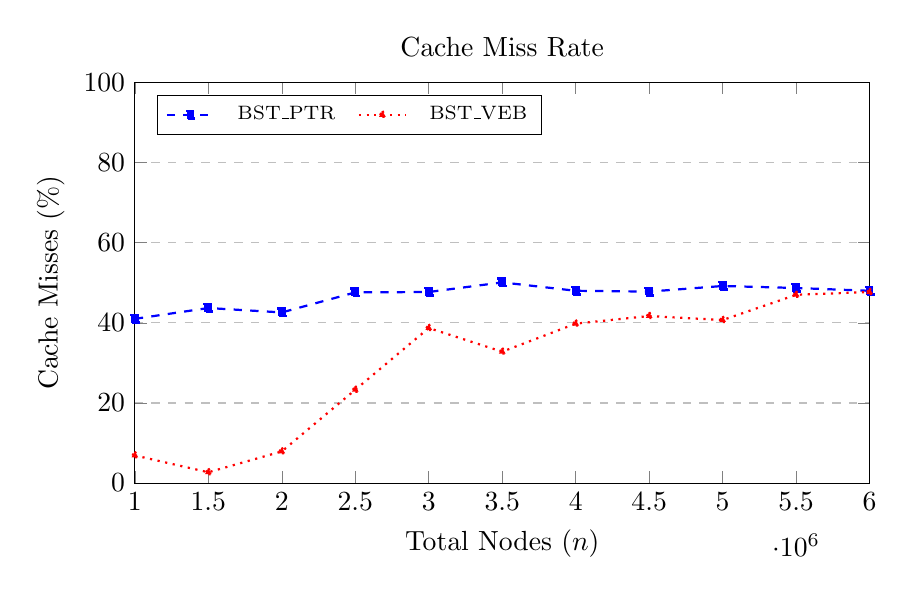
\begin{tikzpicture}
    \begin{axis}[
        title={Cache Miss Rate},
        xlabel={Total Nodes ($n$)},
        ylabel={Cache Misses (\%)},
        width=0.9\textwidth,
        height=0.55\textwidth,
        xmin=1000000, xmax=6000000,
        ymin=0, ymax=100,
        ymajorgrids,
        grid style=dashed,
        legend columns=2,
        legend pos=north west,
        legend style={font=\scriptsize, column sep=6pt},
    ]

    \addplot+[blue, thick, dashed, mark=square*, mark options={scale=.7,fill=blue}]
      coordinates {
        (1000000,41.0) (1500000,43.7) (2000000,42.6) (2500000,47.6)
        (3000000,47.7) (3500000,50.1) (4000000,48.0) (4500000,47.8)
        (5000000,49.2) (5500000,48.7) (6000000,48.0)
      };
    \addlegendentry{BST\_PTR}

    \addplot+[red, thick, dotted, mark=triangle*, mark options={scale=.7,fill=red}]
      coordinates {
        (1000000,6.9) (1500000,2.7) (2000000,7.9) (2500000,23.3)
        (3000000,38.7) (3500000,32.8) (4000000,39.8) (4500000,41.7)
        (5000000,40.7) (5500000,47.0) (6000000,47.7)
      };
    \addlegendentry{BST\_VEB}

    \end{axis}
  \end{tikzpicture}
  \caption{Cache miss rate (\%) as a function of total nodes and lookups ($q=1000000$) for the pointer-based (\texttt{BST\_PTR}) and VanEmde-Boas (\texttt{BST\_VEB}) implementations.}
  \label{fig:cachemissbig}
\end{figure}
